


\documentclass[11pt, a4paper]{article}
%\usepackage{proj1}
\usepackage{natbib}
\usepackage{fancyhdr}  
\usepackage{subcaption}
\usepackage{caption}
\usepackage{graphicx}
\usepackage{numprint}
\usepackage{multirow}
\linespread{1.25} 
\setlength{\parindent}{0cm}
\graphicspath{{Images/}}
\usepackage{hyperref}
\usepackage{amsmath}
\usepackage{amsfonts}
\usepackage{amssymb}
\usepackage{amsthm}
\usepackage{mathtools}
\usepackage{commath}
\usepackage{bbm}

%\usepackage[sc,osf]{mathpazo}
\usepackage{subcaption}
\usepackage[a4paper, top=1in, left=1.0in, right=1.0in, bottom=1in, includehead, includefoot]{geometry} %Usually have top as 1in

\usepackage{listings}
\usepackage{color} %red, green, blue, yellow, cyan, magenta, black, white
\definecolor{mygreen}{RGB}{28,172,0} % color values Red, Green, Blue
\definecolor{mylilas}{RGB}{170,55,241}


\hypersetup{colorlinks,linkcolor={black},citecolor={blue},urlcolor={black}}
\usepackage{color}
\urlstyle{same}


\theoremstyle{definition}
\newtheorem{definition}{Definition}[section]

\newcommand{\adja}{q_a}
\newcommand{\adjb}{q_b}
\newcommand{\adjaB}{q_{a,\partial \Omega}}
\newcommand{\adjbB}{q_{b,\partial \Omega}}
\newcommand{\adjB}{q_{\partial \Omega}}
\newcommand{\Adja}{\mathbf{p}}
\newcommand{\Adjb}{q}
\newcommand{\adj}{q}
\newcommand{\Adjc}{{q}_{\partial \Omega}}
\newcommand{\ra}{\rho_a}
\newcommand{\rb}{\rho_b}
\newcommand{\w}{\mathbf{w}}
\newcommand{\f}{\mathbf{f}}
\newcommand{\ve}{\mathbf{v}}
\newcommand{\n}{\mathbf{n}}
\newcommand{\h}{\mathbf{h}}
\newcommand{\K}{\mathbf{K}}
\newcommand{\hr}{\widehat \rho}
\newcommand{\jf}{\mathbf j}

\DeclareMathOperator{\sgn}{sgn}
\DeclareMathOperator{\Grad}{Grad}
\DeclareMathOperator{\Div}{Div}
\DeclareMathOperator{\Lap}{Lap}
%	\begin{figure}[h]
%		\centering
%		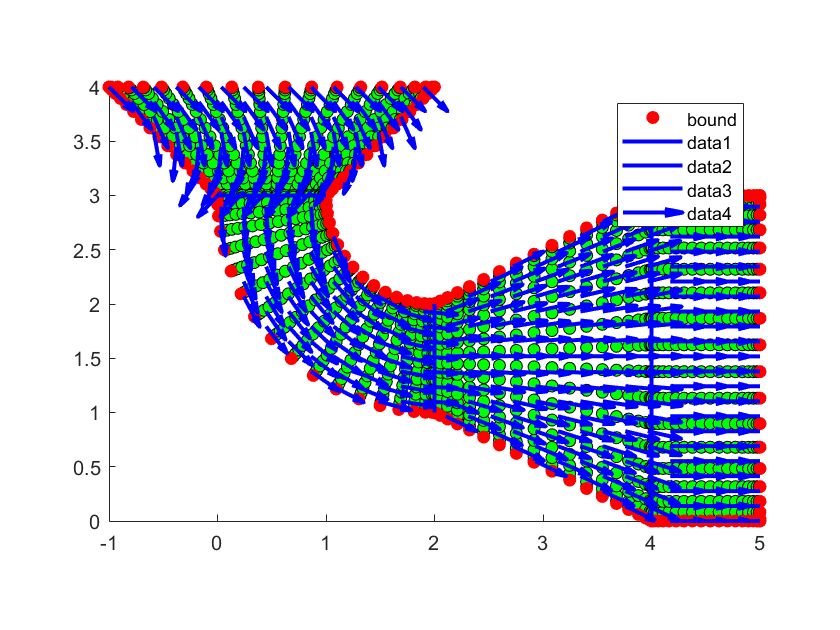
\includegraphics[scale=0.35]{F1.png}
%		\caption{Forward $\rho$ for $a = 0.01$} 
%		\label{F1}
%	\end{figure}

% \item [$\square$]

\begin{document}





\begin{figure}[h]
	\centering
	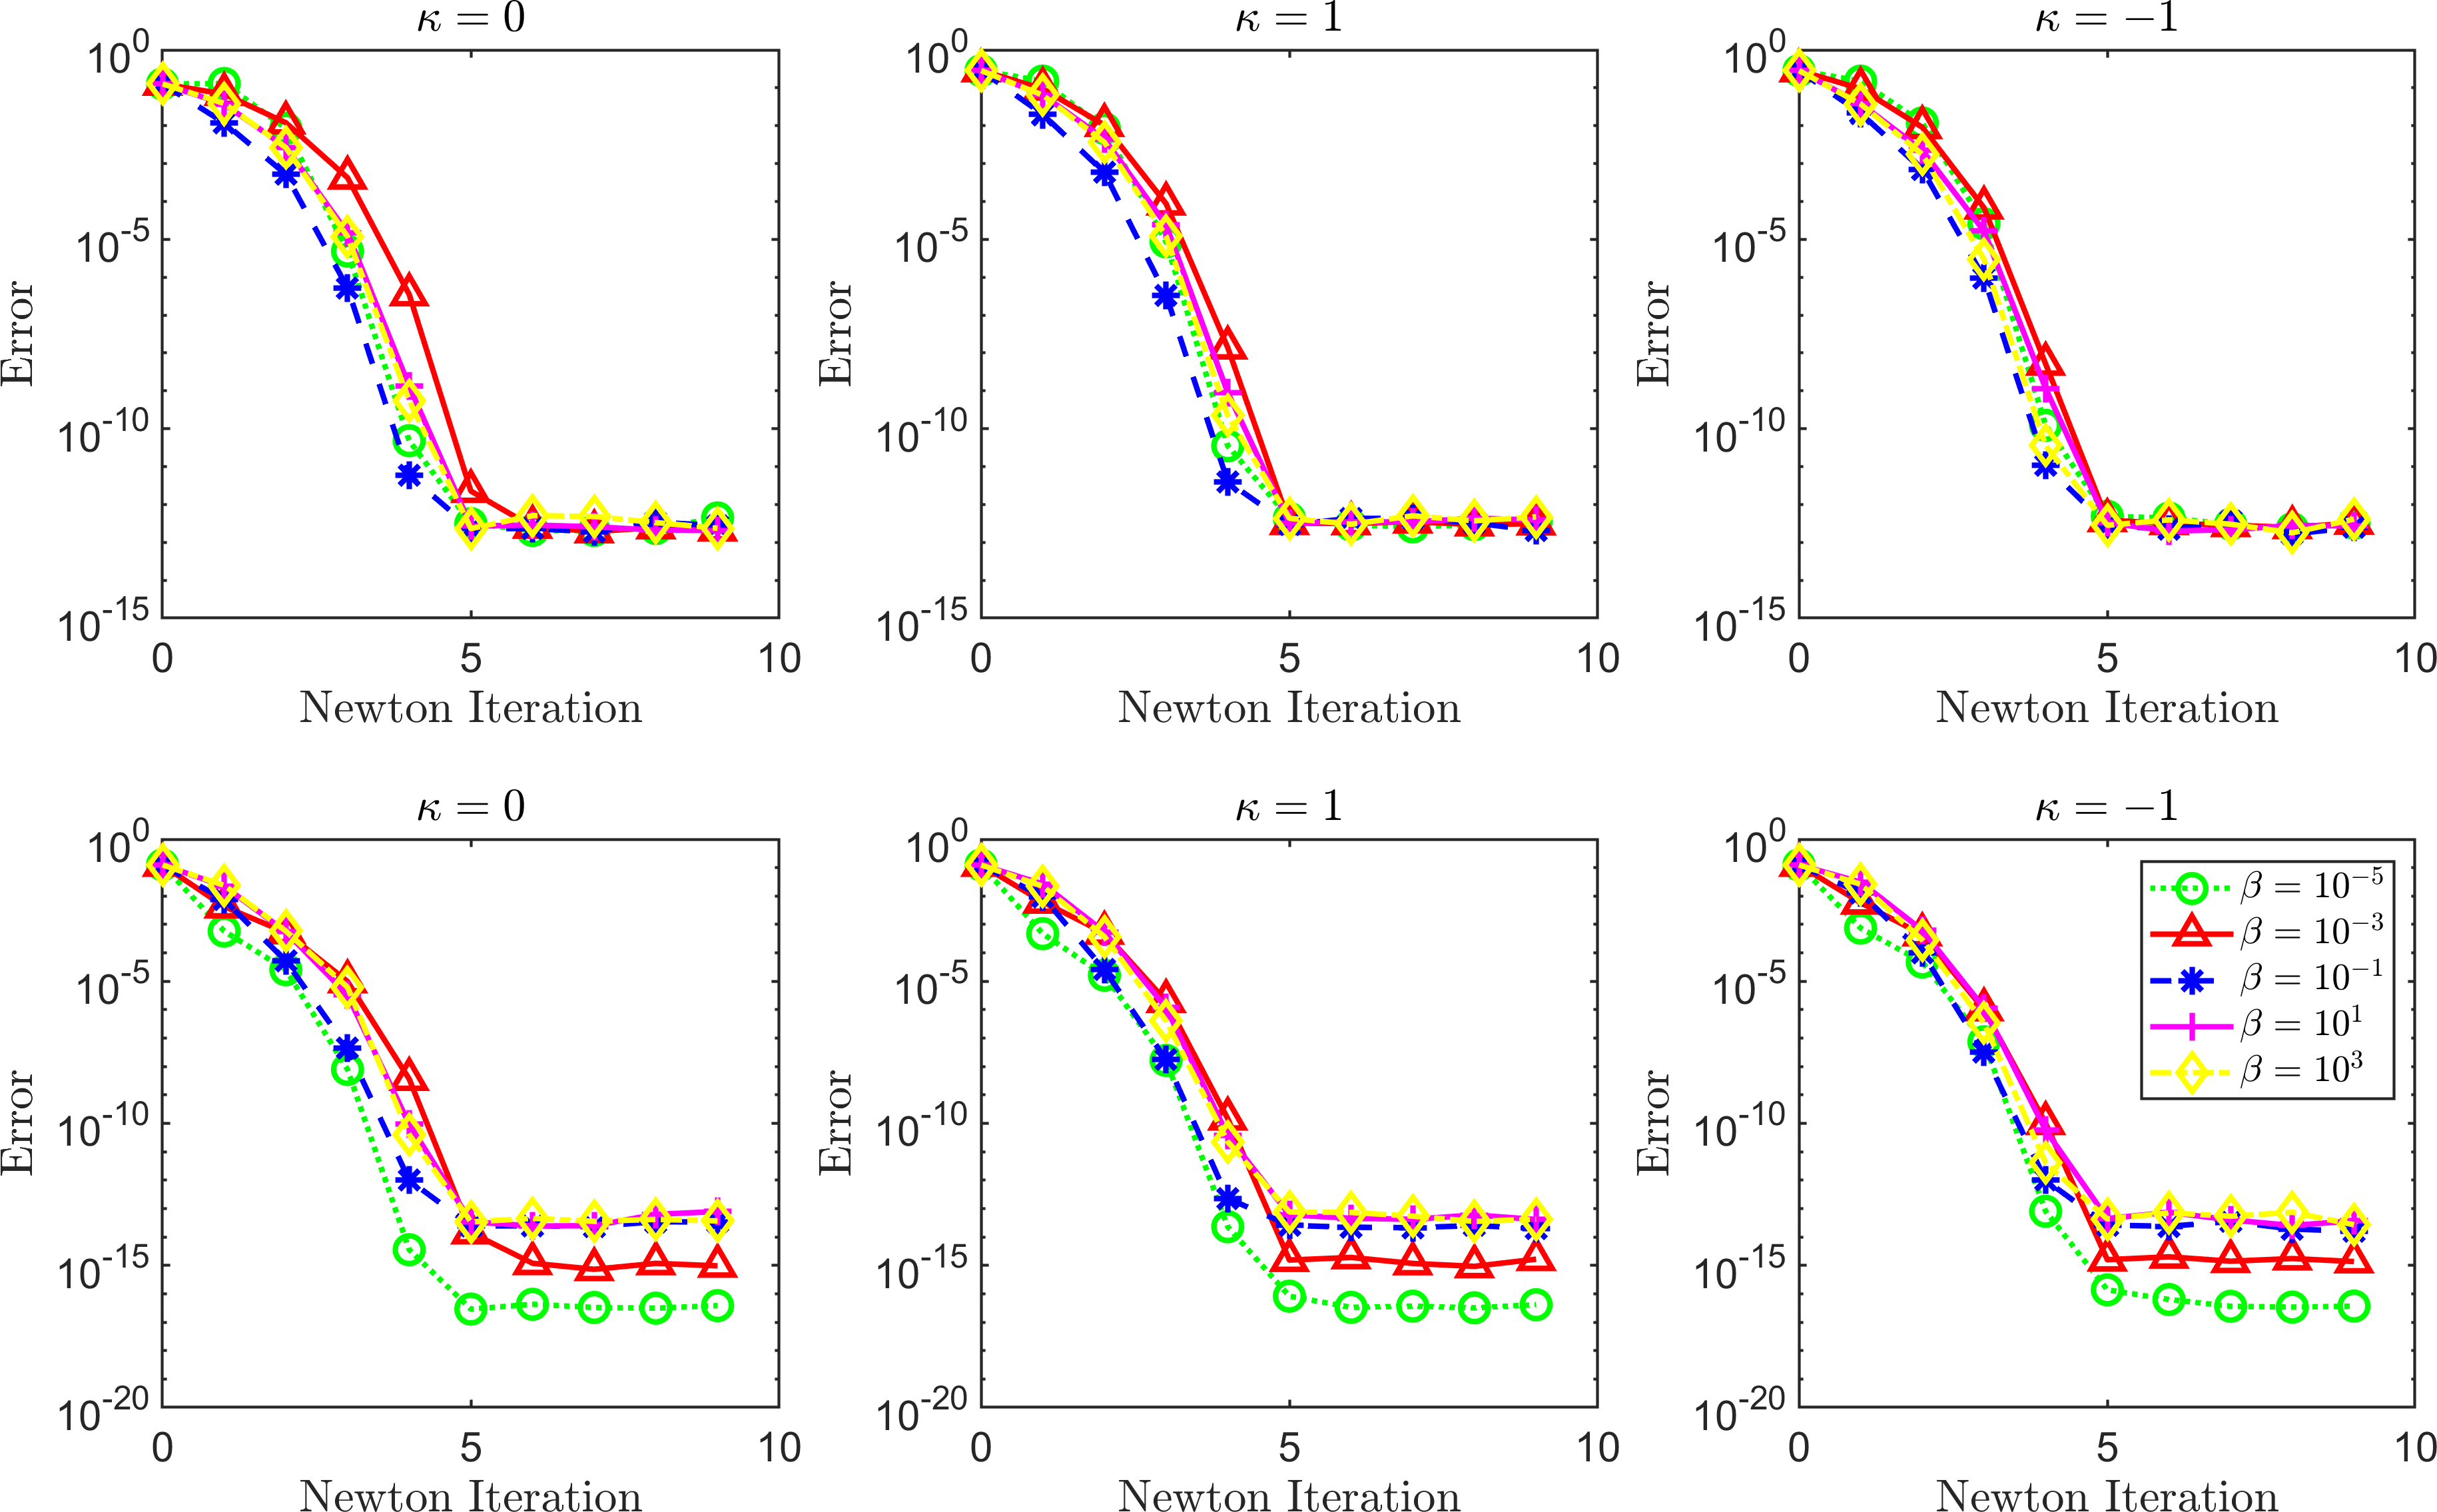
\includegraphics[scale=0.1]{SCNConvergence.png}
	\caption{Convergence of the Newton-Krylov Algorithm for no-flux source control. Top three plots show the convergence in the state variable for different $\kappa$, while the bottom plots show the convergence in the adjoint variable.} 
	\label{Con1}
\end{figure}
\begin{figure}[h]
	\centering
	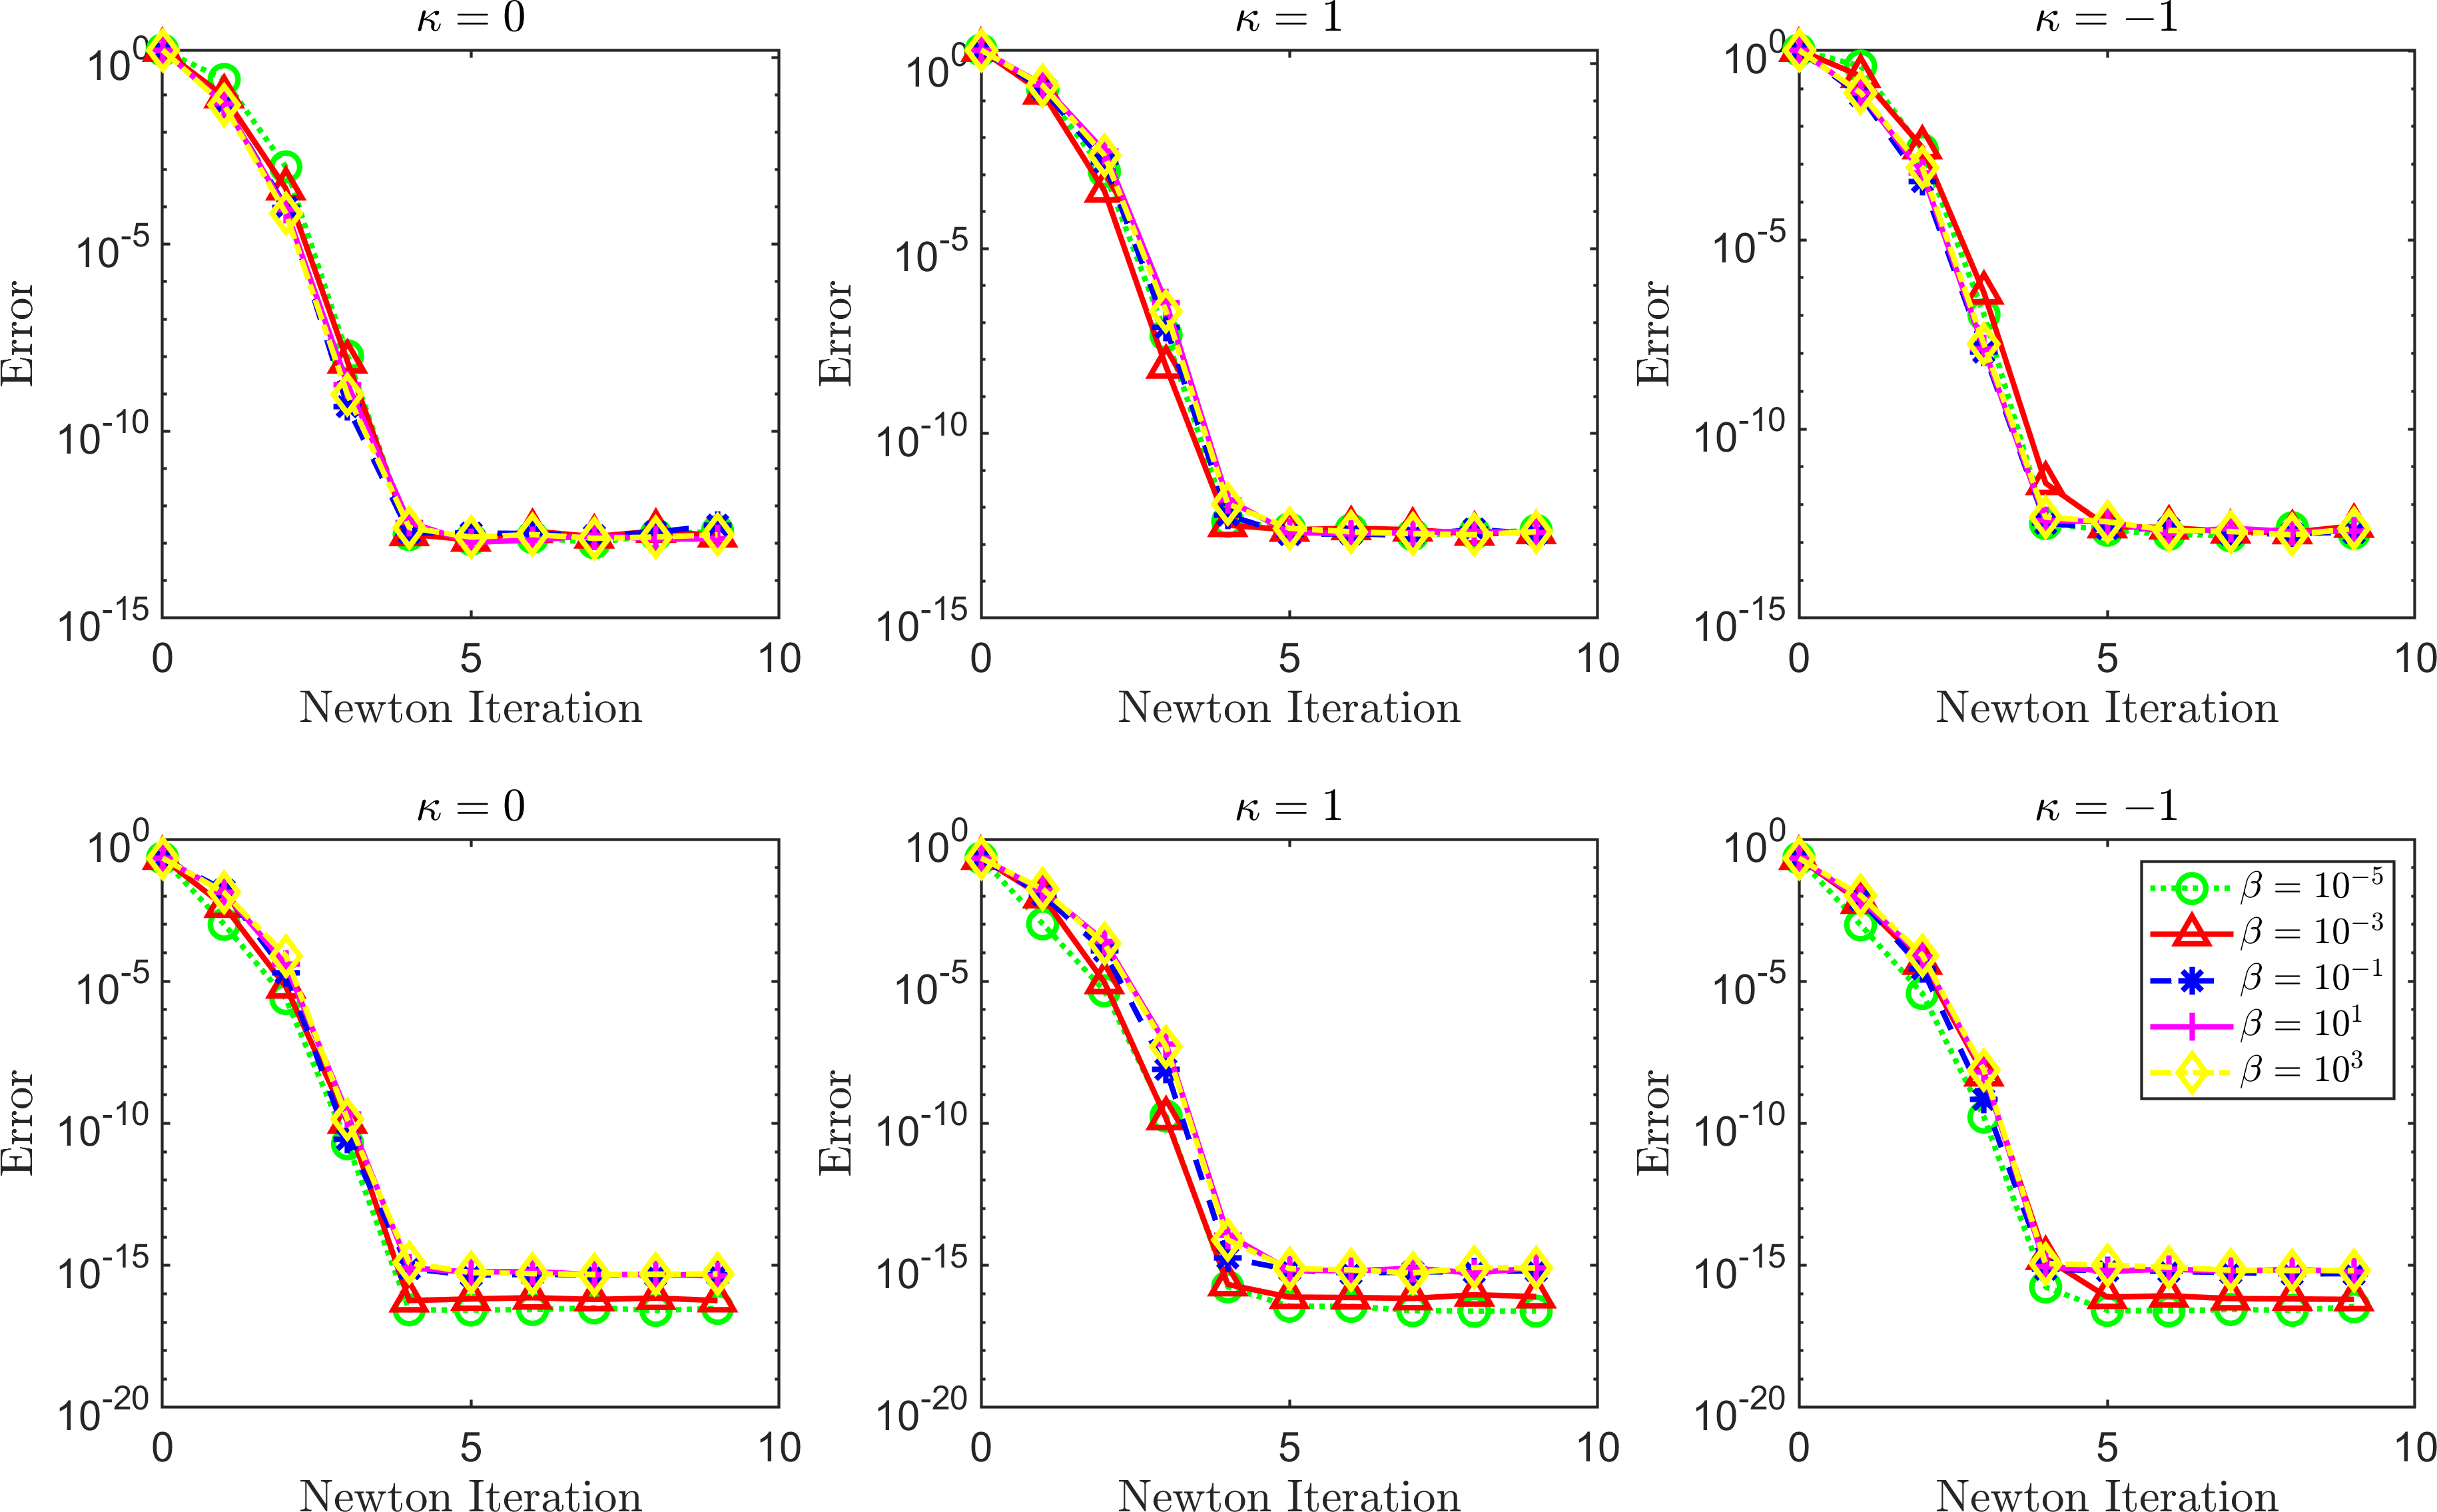
\includegraphics[scale=0.1]{SCDConvergence.png}
	\caption{Convergence of the Newton-Krylov Algorithm for Dirichlet source control. Top three plots show the convergence in the state variable for different $\kappa$, while the bottom plots show the convergence in the adjoint variable.} 
	\label{Con2}
\end{figure}
\begin{figure}[h]
	\centering
	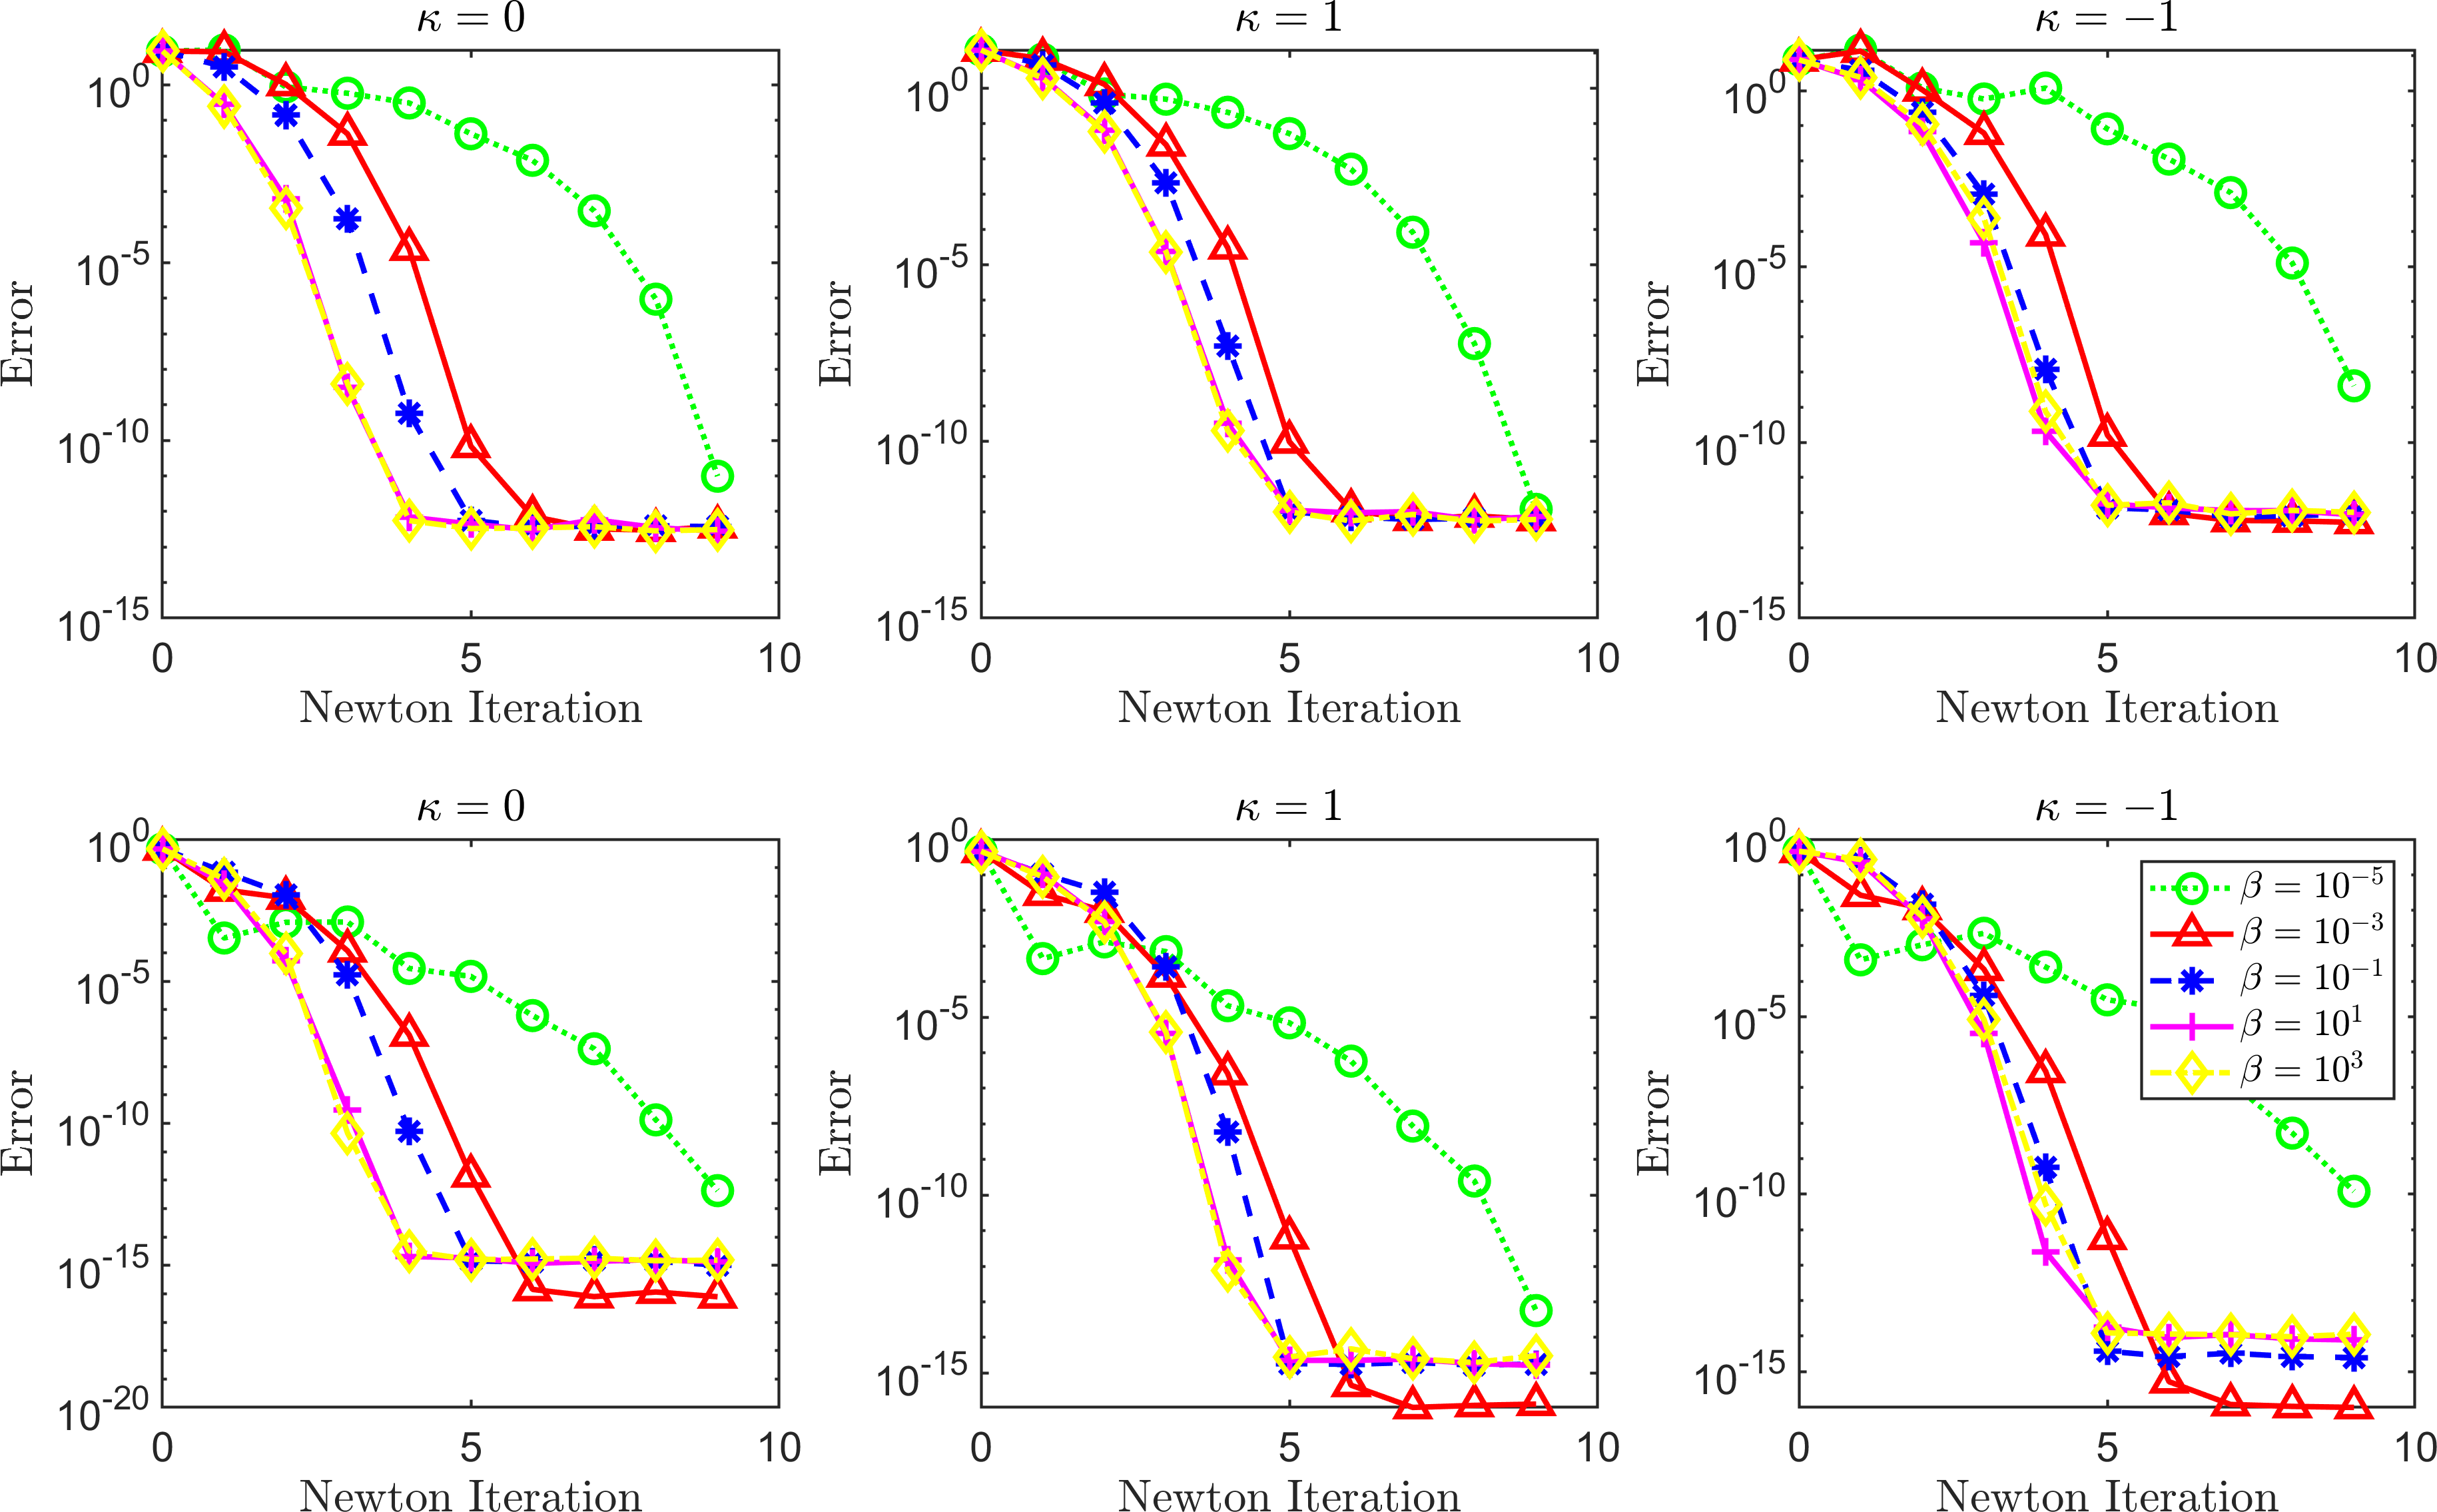
\includegraphics[scale=0.1]{FCDConvergence.png}
	\caption{Convergence of the Newton-Krylov Algorithm for Dirichlet flow control. Top three plots show the convergence in the state variable for different $\kappa$, while the bottom plots show the convergence in the adjoint variable.} 
	\label{Con3}
\end{figure}
\begin{figure}[h]
	\centering
	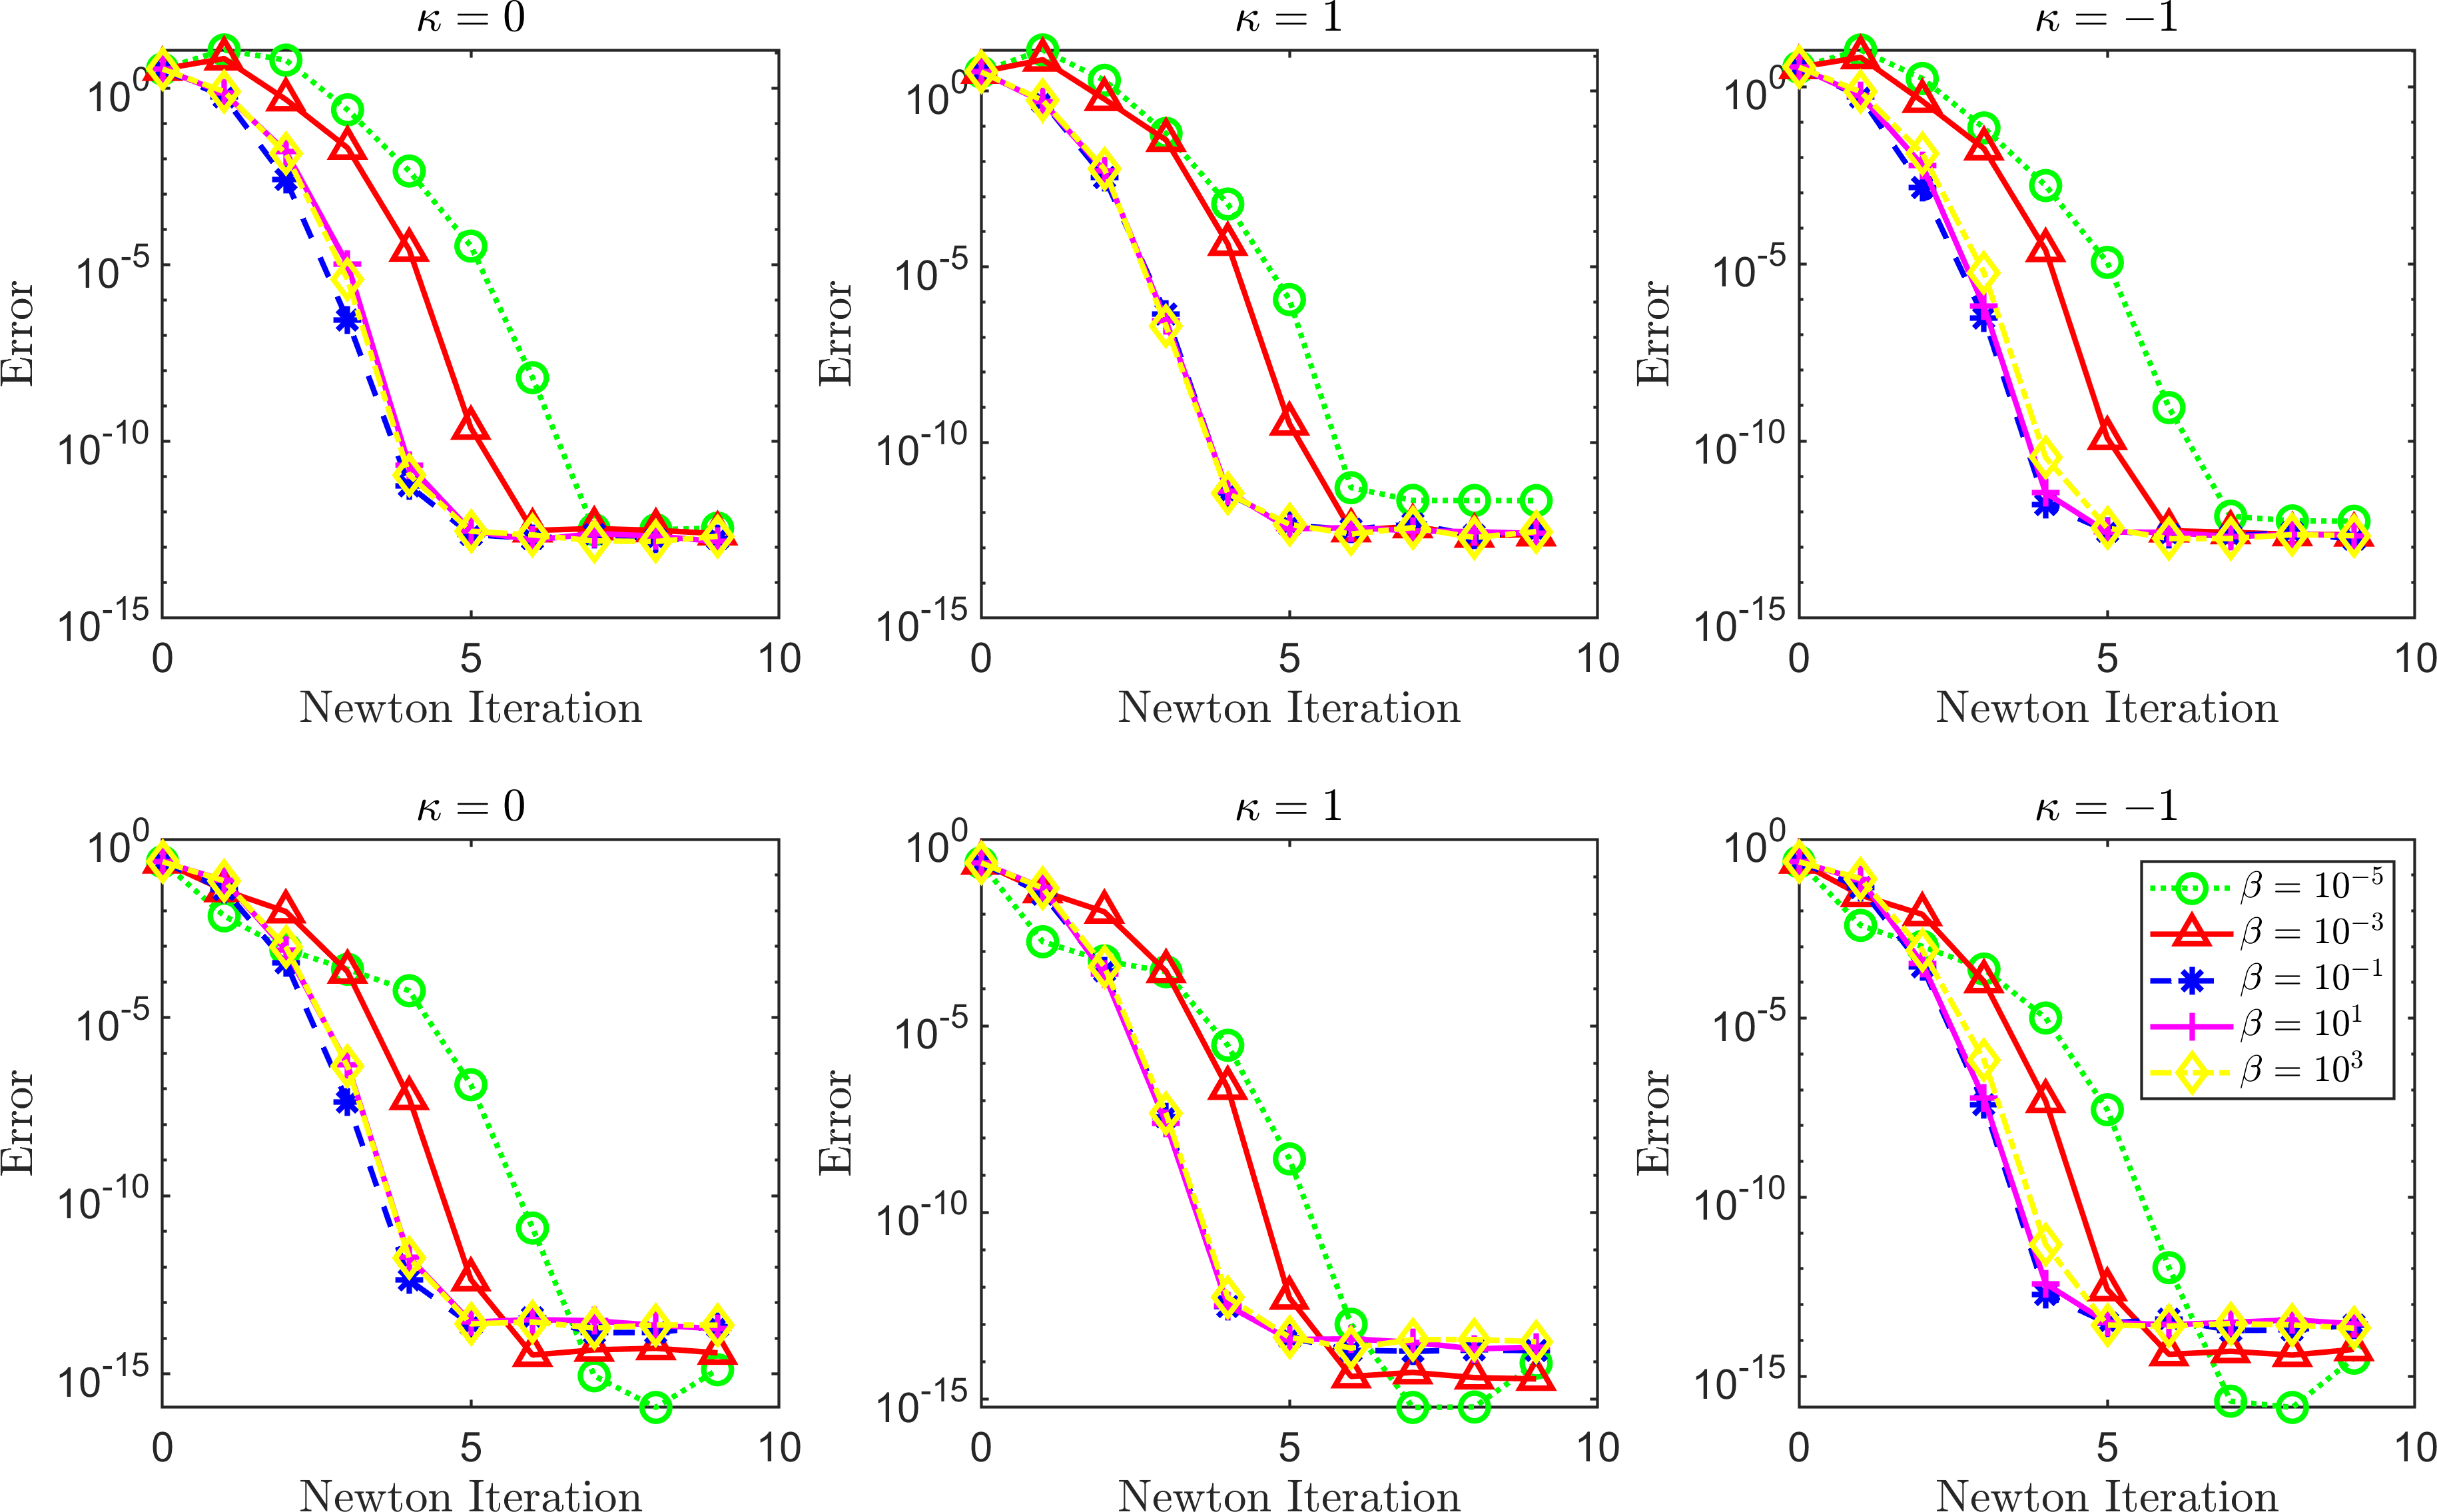
\includegraphics[scale=0.1]{FCNConvergence.png}
	\caption{Convergence of the Newton-Krylov Algorithm for no-flux flow control. Top three plots show the convergence in the state variable for different $\kappa$, while the bottom plots show the convergence in the adjoint variable.} 
	\label{Con4}
\end{figure}





\end{document}